\documentclass[crop=false]{standalone}
\usepackage{standard}

\begin{document}
  \section{Hilfsmittel und Entwicklungsumgebung} % (fold)
  \label{sec:Hilfsmittel und Entwicklungsumgebung}

  Ein wesentlicher Bestandteil für die Bearbeitung der Aufgabenstellungen war die Einrichtung einer passenden Entwicklungsumgebung.
  Diese sollte einen effizienten Arbeitsfluss ermöglichen und die Zusammenarbeit mit anderen Teams vereinfachen.
  Hierfür verwendete ich sowohl Methoden, die ich durch meine Tätigkeit am Fraunhofer ITWM erlangte, als auch Herangehensweisen, welche mir aus Vorlesungen bekannt waren.

  \subsection{Versionsverwaltung mit Git} % (fold)
  \label{sub:git}
    Ein typisches Werkzeug für eine Entwicklungsumgebung ist ein Versionskontrollsystem (VCS).
    Es protokolliert die Änderungen gegebener Dateien im Verlauf der Zeit.
    Auf jeden protokollierten Zeitpunkt (engl.: \textit{commit}) kann zugegriffen werden, sodass auch nach dem Löschen von Informationen diese immer noch abrufbar sind.
    Ein VCS stellt damit eine effiziente Alternative des herkömmlichen Backups dar.
    Die Aufgabe des VCS wurde in meinem Projekt durch das Programm \textit{Git} übernommen.
    Es ist ein verteiltes Open-Source-VCS, welches durch seine Arbeitsweise verschiedene Vorteile gegenüber anderen Systemen aufweist.

    Mit \textit{Git} erstellte ich für jedes meiner Projekte ein sogenanntes Archiv (engl.: \textit{repository}).
    Diese Archive beinhalteten ein derzeitiges Arbeitsverzeichnis, sowie alle protokollierten Zeitpunkte mit deren zugehörigem Inhalt.
    Um diese auf mehreren Rechnersystemen bearbeiten zu können, verwendete ich die bekannten öffentlichen \textit{Git}-Server \textit{GitHub} und \textit{GitLab}.

    Um anderen Entwicklern das Verstehen meiner geleisteten Arbeit zu vereinfachen, strukturierte ich mein Projekt nach festen Regeln.
    \textit{Commit}-Nachrichten, die jedem protokollierten Zeitpunkt eine Bedeutung gaben, mussten ein spezielles Format aufweisen%
    \footnote{https://chris.beams.io/posts/git-commit/}.
    Abbildung \ref{fig:commit-message-example} zeigt die Verwendung dieses Formats anhand eines realen Beispiels.
    \begin{figure}
      \center
      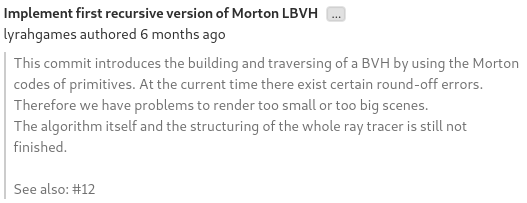
\includegraphics[width=0.7\textwidth]{images/commit_message_example.png}
      \caption{%
        Die Abbildung zeigt das Format von \textit{Commit}-Nachrichten anhand eines realen Beispiels.
        Es existiert eine Überschrift im Imperativ und optional eine Erläuterung und Referenzen auf bereits dokumentierte Probleme.
      }
      \label{fig:commit-message-example}
    \end{figure}

    \textit{Commits} in \textit{Git} werden zudem noch auf unterschiedliche Verzweigungen (engl.: \textit{branches}) aufgeteilt.
    Dies ermöglicht die Bearbeitung des Quelltextes an mehreren Stellen gleichzeitig.
    Durch das Verschmelzen (engl.: \textit{merge}) zweier Verzweigungen lassen sich Änderung von einer Verzweigung in eine andere überführen.
    Eine unsystematische Verwendung von \textit{Branches} führt bei einem \textit{Merge} im Normalfall jedoch zu fehlerbehafteten Artefakten im Quelltext.
    Aus diesem Grund wurden in den hier gezeigten Projekten \textit{Branches} nur auf spezielle Weise verwendet.
    Ich richtete mich vor allem nach dem bekannten \textit{git-flow}-Modell%
    \footnote{http://nvie.com/posts/a-successful-git-branching-model/}, %
    bei welchem die eigentliche Entwicklung auf einer \textit{Develop}-\textit{Branch} und mehreren \textit{Feature}-\textit{Branches} vollzogen wird.
    Bei Veröffentlichungen von neuen Versionen werden \textit{Master}- und \textit{Release}-\textit{Branches} verwendet.
    Abbildung \ref{fig:git-flow-example} zeigt dieses Modell wieder anhand eines realen Beispiels.
    \begin{figure}
      \center
      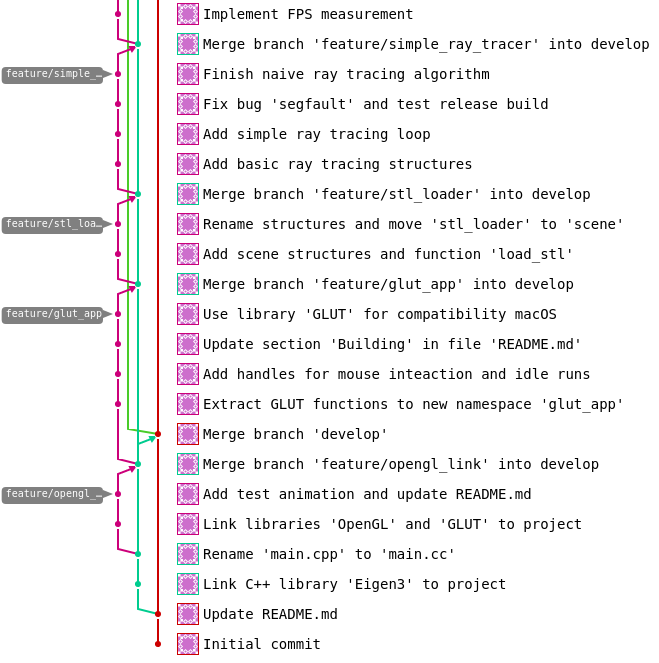
\includegraphics[width=0.7\textwidth]{images/git_flow_example.png}
      \caption{%
        Die Abbildung zeigt ein Beispiel für die Anwendung des git-flow-Modells anhand eines durch \textit{GitLab} erstellten Graphen.
        Es handelt sich um die reale Entwicklungsgeschichte (engl.: \textit{History}) des hier behandelten Projekts.
        Jeder mit Text beschriftete Eintrag stellt einen protokollierten Zeitpunkt dar.
        Der Graph auf der linken Seite zeigt den zugehörigen Verzweigungsbaum (engl.: \textit{commit tree}).
      }
      \label{fig:git-flow-example}
    \end{figure}
  % subsection git (end)


  \subsection{CMake} % (fold)
  \label{sub:cmake}
    Die Verwendung unterschiedlicher Hardware und Betriebssysteme stellt häufig ein Hindernis bei der Entwicklung robusten Quellcodes dar.
    Aus diesem Grund verwendete ich innerhalb meiner Projekte CMake.
    Es ist ein Build-System-Generator.
    Durch die Ausführung von CMake wird ein entsprechendes Build-System konfiguriert, welches sich dem zugrundeliegenden Rechnersystem anpasst.
    Das erzeugte Build-System ist in der Lage den Quellcode mit seinen Abhängigkeiten zu kompilieren und auch zu testen.
    Mittlerweile stellt es eines der Standardwerkzeuge für jeden C- und C++-Programmierer dar.

    Um auch hier für andere Entwickler eine feste Struktur beizubehalten, stützte ich mich für das Schreiben von CMake-Dateien auf die zugehörige Dokumentation%
    \footnote{https://cmake.org/documentation}.
    Somit konnte ich moderne Standards lernen und anwenden.
    Die CMake-Dateien beschrieben dadurch immer die benötigten Anforderungen, um den Quelltext fehlerfrei zu kompilieren.
  % subsection cmake (end)

  \subsection{C/C++-Compiler} % (fold)
  \label{sub:c_c_compiler}
    Natürlich wird für die Kompilierung von Quellcode auch ein entsprechender Compiler benötigt.
    Das Ziel war es, den geschriebenen Code mit verschiedenen Compilern, wie zum Beispiel \textit{GCC}, \textit{Clang} und dem \textit{Intel C++ Compiler}, übersetzen zu können.
    Dies sollte sicherstellen, dass innerhalb des Quelltextes keine Compiler-internen Konstrukte verwendet wurden, die auf anderen Systemen vielleicht nicht existierten.
  % subsection c_c_compiler (end)

  \subsection{Weitere Hilfsmittel} % (fold)
  \label{sub:weitere_hilfsmittel}
    Um Quelltext zu kreieren wird ein Texteditor oder sogar eine integrierte Entwicklungsumgebung (IDE, engl.: \textit{integrated development environment}) benötigt.
    Ich verwendete den Editor \textit{Sublime Text}%
    \footnote{https://www.sublimetext.com}, der als eine Mischung zwischen Texteditor und IDE angesehen werden kann.
    Er bietet viele Funktionalitäten einer IDE, arbeitet jedoch effizienter durch seine geringere Nutzung des Arbeitsspeichers.
    Zudem erlaubt \textit{Sublime Text} durch eine eigene Paketverwaltung das Installieren weiterer Funktionalitäten.
    Abbildung \ref{fig:sublime-text-example} zeigt \textit{Sublime Text} im Einsatz.
    \begin{figure}
      \center
      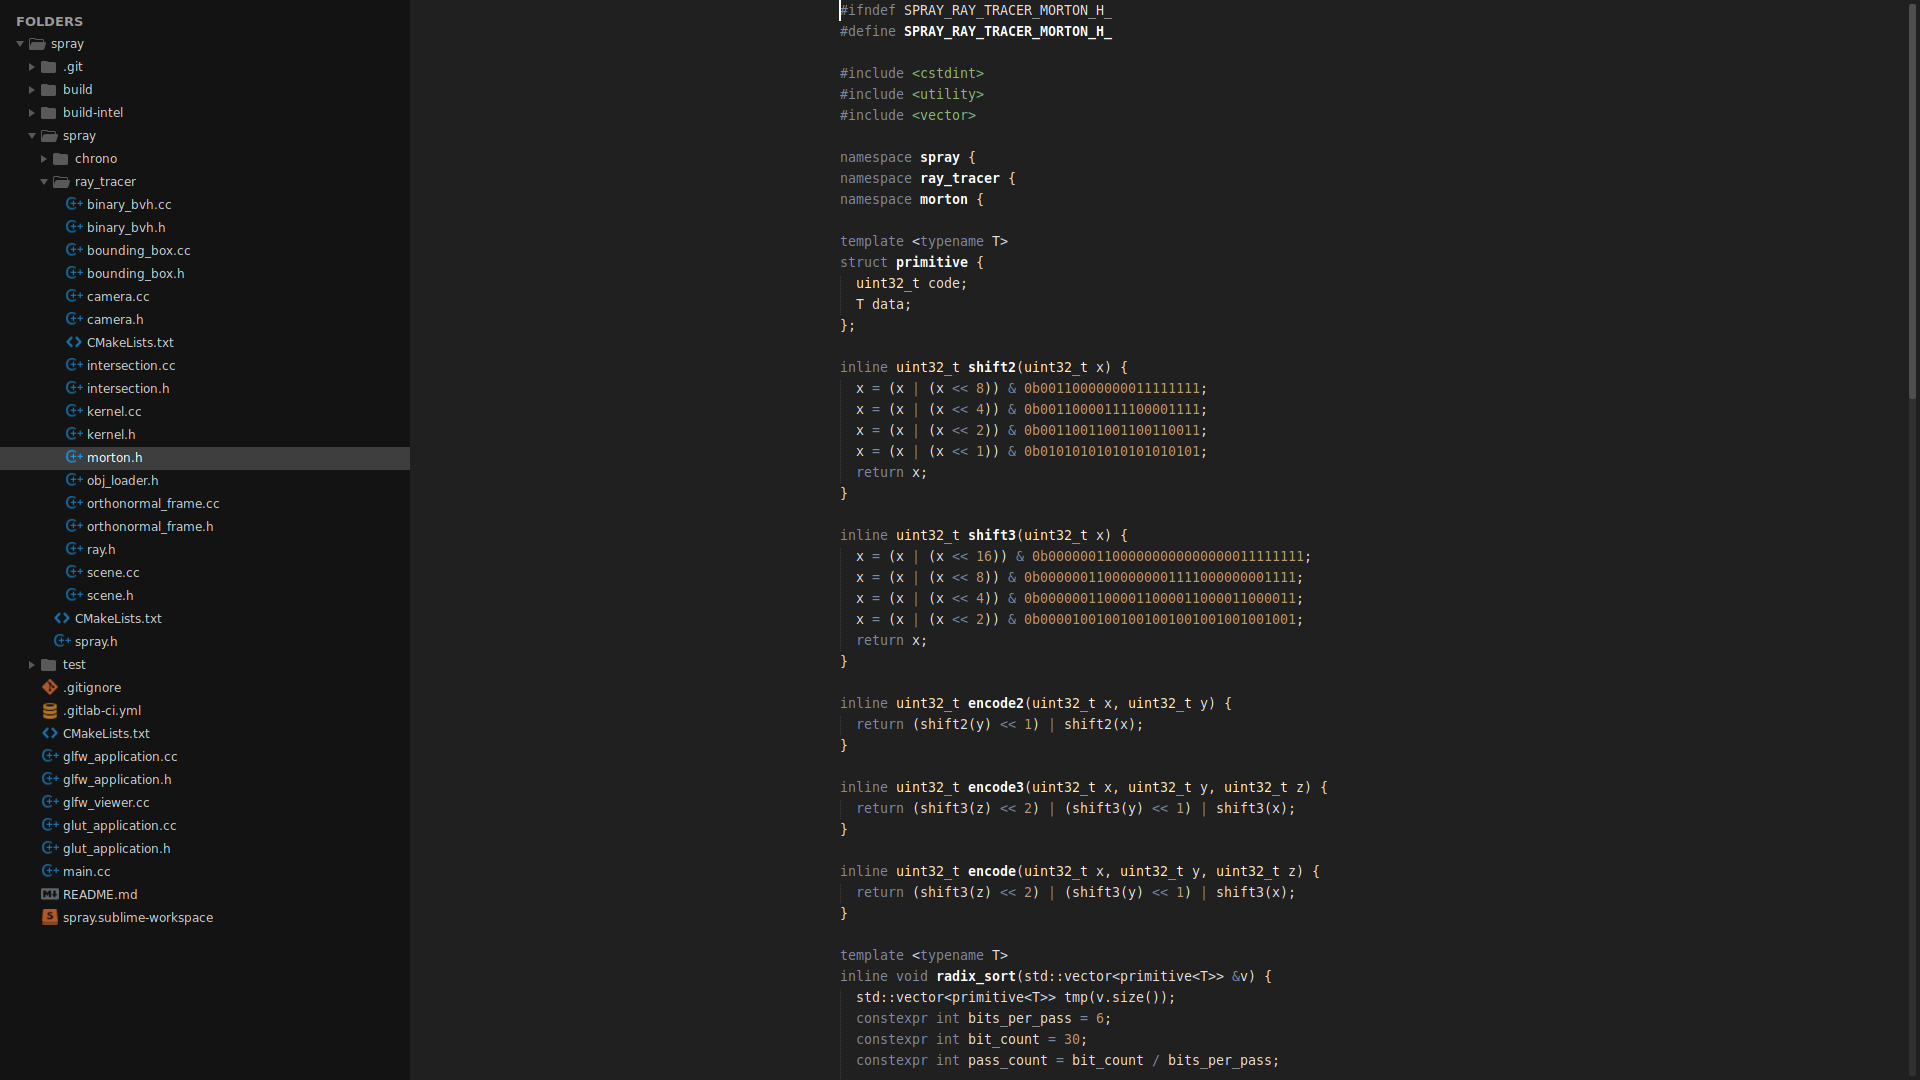
\includegraphics[width=0.8\textwidth]{images/sublime_text_example.png}
      \caption{%
        Die Abbildung zeigt den Editor \textit{Sublime Text} mit dem hier bearbeiteten Projekt.
        Die linke Seite zeigt die sogenannte \textit{Sidebar} mit dem Verzeichnisbaum des Projekts.
      }
      \label{fig:sublime-text-example}
    \end{figure}

    Das Schreiben von Quelltext beinhaltet auch die Formatierung dessen.
    Eines der größten Probleme in der Softwareentwicklung besteht darin, fremden Quelltext zu lesen und zu verstehen.
    Durch \textit{Style Guides} werden dem Programmierer Orientierungshilfen für die Formatierung des Codes und die Beantwortung von Stilfragen geboten.
    Die Verwendung von \textit{Style Guides} ermöglicht ein besseres Code-Verständnis innerhalb einer Projektgruppe.
  % subsection weitere_hilfsmittel (end)

  % section entwicklungsumgebung (end)
\end{document}